%%%%%%%%%%%%%%%%%%%%%%%%%%%%%%%%%%%%%%%%%%%%%%%%%%%%%%%%%%%%%%%%%%%%%%%%%
%
% File: operator_evolution.tex
%
% Author: A. J. Tropiano (tropiano.4@osu.edu)
% Date: August 23, 2019
%
% Draft of paper on SRG operator evolution and the Magnus expansion.
%
% Revision history:
%	...
%
%%%%%%%%%%%%%%%%%%%%%%%%%%%%%%%%%%%%%%%%%%%%%%%%%%%%%%%%%%%%%%%%%%%%%%%%%


\documentclass[preprintnumbers,floatfix,aps,prc,preprint,nofootinbib]{revtex4-1}

% Packages
\usepackage{amsmath}
\usepackage{amsfonts}
\usepackage{amssymb}
\usepackage{bm}
\usepackage[font=small,skip=0pt]{caption} % For captions on figures and tables
\usepackage{cellspace}
\usepackage{color}
\usepackage{enumerate}
\usepackage{epsfig}
\usepackage[figuresright]{rotating}
\usepackage{float}
\usepackage{hyperref} % For clickable links to sections within table of contents
\usepackage{graphicx}
\graphicspath{{../../Figures/Operator_evolution/}} % Setting the graphics path
\graphicspath{{../../Figures/SRG_operator_evolution/}}
\usepackage{physics} % For bra-ket notation
\usepackage{siunitx}
\usepackage[caption=false]{subfig} % For sub-figures

\newcommand{\eps}{\varepsilon}


\begin{document}


%%%%%%%%%%%%%%%%%%%%%%%%%%%%%%%%%%%%%%%%%%%%%%%%%%%%%%%%%%%%%%%%%%%%%%%%%
\title{Operator evolution from the similarity renormalization group and the Magnus expansion}


\author{A.~J.~Tropiano$^{1}$, S.~K.~Bogner$^{2}$, R.~J.~Furnstahl$^{1}$}

\affiliation{%
		$^1$\mbox{Department of Physics, The Ohio State University, Columbus, OH 43210, USA}  \\
		$^2$\mbox{National Superconducting Cyclotron Laboratory and Department of Physics and Astronomy,}  \\
    		\mbox{Michigan State University, East Lansing, MI 48824, USA}
}

\date{\today}

\begin{abstract}

\noindent{Ideas for Magnus / SRG operator evolution paper}
\\
-- SRG/Magnus evolution in different potentials (non-local, local, semi-local). Universality. High cutoffs.
\\
-- Block-diagonal generator for high cutoff potentials and operator evolution. How the block-diagonal generator handles spurious bound states.
\\
-- Testing the Magnus expansion for high cutoff potentials using the potentials from Wendt 2011 for comparison. Spurious bound states and connection to intruder states in IMSRG calculations.
\\
-- Operator evolution for different potentials and generators.

\end{abstract}

\maketitle

\newpage


%%%%%%%%%%%%%%%%%%%%%%%%%%%%%%%%%%%%%%%%%%%%%%%%%%%%%%%%%%%%%%%%%%%%%%%%%
\section{Introduction}
\label{sec:intro}


\noindent{%
\textbf{Background on modern nuclear potentials.}
}
\\
-- Wide range of NN potentials: how do they change under SRG transformations?
\\
-- Implementation to many-body calculations and SRG decoupling.
\\
-- Motivate long list of unaddressed questions: regulator, generator dependence, universality, high cutoffs, the Magnus expansion.
\\
\textbf{SRG formalism}
\\
-- The SRG decouples low- and high-momentum scales by applying a continuous unitary transformation $U(s)$ where $s=0 \rightarrow \infty$ is the flow parameter.
\\
-- The `dressed' or evolved operator is given by
%
\begin{eqnarray}
	\label{eq:srg_operator}
	O(s) = U(s) O(0) U^{\dagger}(s),
\end{eqnarray}
%
where $O(0)$ corresponds to the `bare' operator.
\\
-- Because $U(s)$ is unitary, the observables of the operator are preserved.
\\
-- In practice, the unitary transformation U(s) is not explicitly solved for; the evolved operator is given by a differential flow equation which is obtained by taking the derivative of Eqn. (\ref{eq:srg_operator}),
%
\begin{eqnarray}
	\label{eq:srg_flow}
	\frac{dO(s)}{ds} = [\eta(s), O(s)],
\end{eqnarray}
%
where $\eta(s)=\frac{dU(s)}{ds} U^{\dagger}(s) = -\eta^{\dagger}(s)$ is the anti-hermitian SRG generator.
\\
-- The generator is defined as a commutator,
%
\begin{eqnarray}
	\label{eq:srg_generator}
	\eta(s) = [G, H(s)],
\end{eqnarray}
%
where $G$ specifies the type of flow or form of the decoupled operator.
\\
-- To drive the operator to band-diagonal form, set $G=H_D(s)$, the diagonal of the Hamiltonian.
\\
-- This choice was implemented by Wegner in condensed matter physics \cite{Wegner:1994ab}.
\\
-- For notational convenience, we write the Wegner choice without the $s$ dependence in the rest of the paper.
\\
-- In a similar option used in nuclear physics, $G$ is set to the relative kinetic energy, $T_{rel}$, which also drives to band-diagonal form.
\\
-- In this paper, we consider both choices.
\\
\textcolor{red}{%
-- Add block-diagonal generator.
}
\\
-- Generally the flow equation (\ref{eq:srg_flow}) is solved up to some finite value of $s$ with a high-order ODE solver.
\\
-- It is convenient to define $\lambda \equiv s^{-1/4}$ which roughly measures the width of the band-diagonal in the decoupled operator.
\\
\textbf{Operator evolution}
\\
-- State how a potential and wave function changes: how does this affect other operators?
\\
-- How operators evolve from band- and block-diagonal SRG transformations.
\\
-- Operator evolution for different potentials (regulators, chiral order, etc.)


%%%%%%%%%%%%%%%%%%%%%%%%%%%%%%%%%%%%%%%%%%%%%%%%%%%%%%%%%%%%%%%%%%%%%%%%%
\section{SRG evolution of NN potentials}
\label{sec:srg_evolution_nn_potentials}


\noindent{%
-- Comparison of potential evolution with different regulators, orders, generators.
}
\\
-- Universality.
\\
-- Discussion of high cutoffs, block-diagonal generator at high cutoffs, and how it handles spurious bound states.
\\
-- Use high cutoffs to transition to Magnus test problem.
\\
-- Example figure. EM N$^3$LO potential.
%
\begin{figure}[H]
	\centering
	\subfloat[]{%
	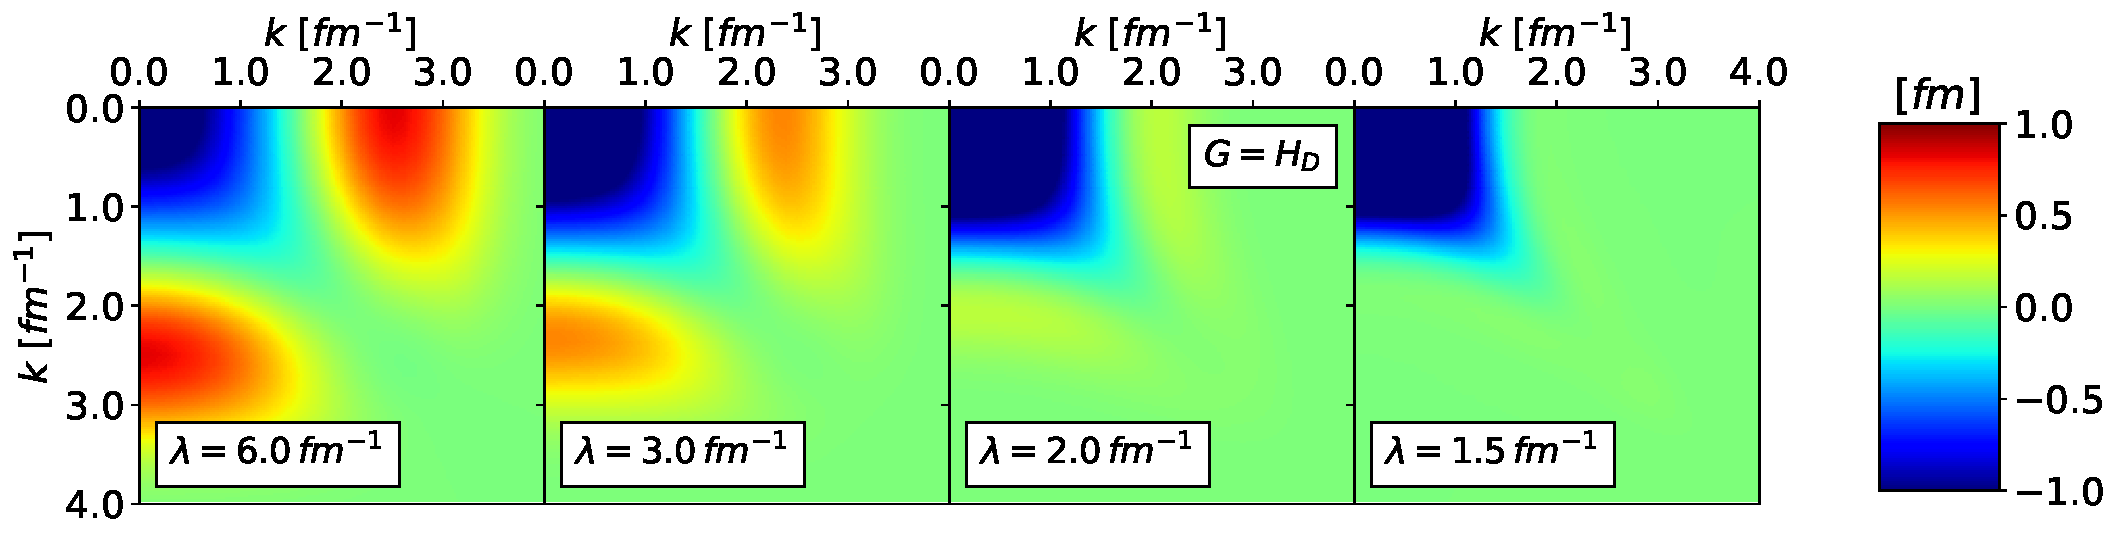
\includegraphics[clip,width=0.9\columnwidth]{potential_contours_kvnn10_3S1_Wegner}%
	}
	
	\subfloat[]{%
	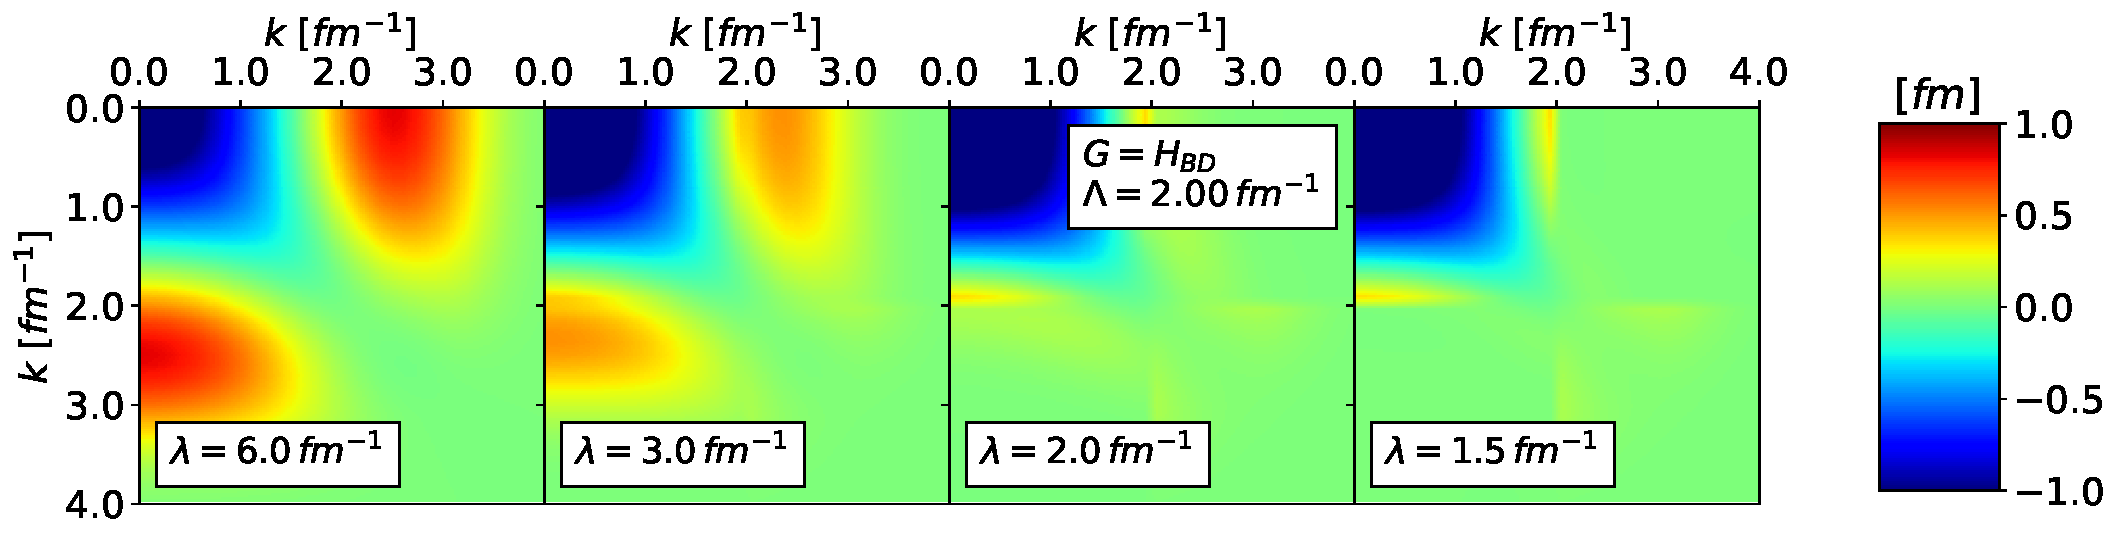
\includegraphics[clip,width=0.9\columnwidth]{potential_contours_kvnn10_3S1_Block-diag2,00}%
	}

	\subfloat[]{%
	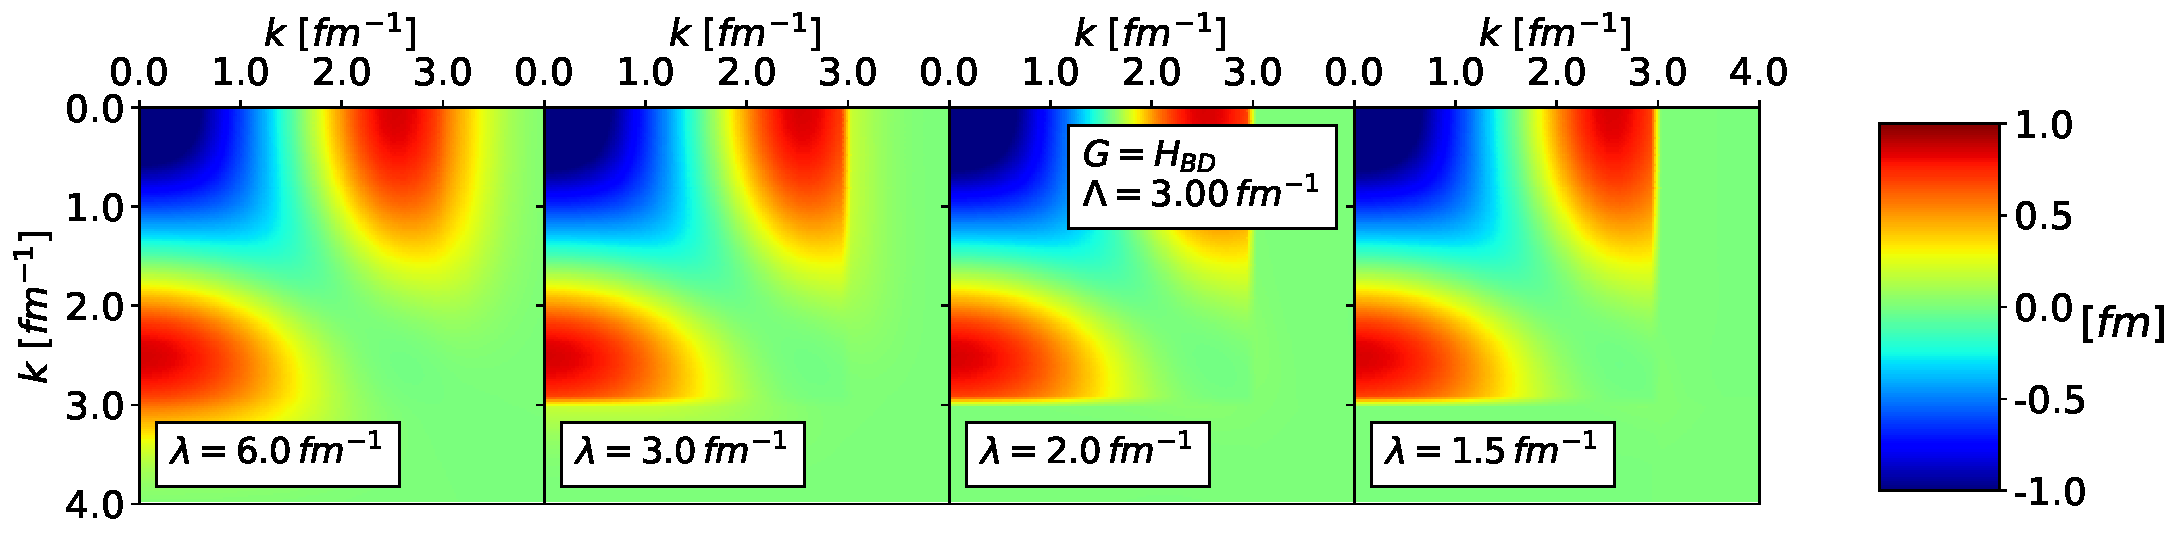
\includegraphics[clip,width=0.9\columnwidth]{potential_contours_kvnn10_3S1_Block-diag3,00}%
	}
	\caption{Matrix elements of the Entem-Machleidt N$^3$LO non-local potential $V_{\lambda}(k, k')$ SRG-evolving in $\lambda$ right to left under transformations with the Wegner generator (a) and block-diagonal generators decoupling at $\Lambda=2$ and $3$ fm$^{-1}$ (b and c).}
	\label{potential_contours_kvnn10_3S1}
\end{figure}


%%%%%%%%%%%%%%%%%%%%%%%%%%%%%%%%%%%%%%%%%%%%%%%%%%%%%%%%%%%%%%%%%%%%%%%%%
\section{The Magnus expansion}
\label{sec:magnus_expansion}


\noindent{%
-- Summary of Wendt high cutoff results and connection to IMSRG intruder state.
}


% - - - - - - - - - - - - - - - - - - - - - - - - - - - - - - - - - - - - - - - - - - - - - - - - - - - - - - - - - - - - - - - - - - - - - - - - - - - - - - - - - - - - - - - - - - - - - - - - - - - - - - - - 
\subsection{Formalism}
\label{sec:magnus_expansion_formalism}


\noindent{%
-- Motivation: simplifies computational problem for evolving multiple operators, exact unitarity.
}
\\
-- We now consider the Magnus implementation.
\\
-- Mathematically speaking, the Magnus expansion is a method for solving an initial value problem associated with a linear ordinary differential equation (ODE).
\\
-- Formal details of the Magnus expansion are discussed in \cite{Blanes:2009ab}.
\\
-- We will introduce the Magnus expansion in the context of SRG evolving any operator.
\\
-- In an intermediate step in deriving Eqn. (\ref{eq:srg_flow}), we have a linear ODE for $U(s)$,
%
\begin{eqnarray}
	\label{eq:unitary_trans}
	\frac{dU(s)}{ds} = \eta(s) U(s).
\end{eqnarray}
%
-- Magnus showed that one can solve the following equation with a solution $U(s)=e^{\Omega(s)}$ where $\Omega(s)$ is expanded as a power series, $\sum_{n}^{\infty} \Omega_n$ (referred to as the Magnus expansion or Magnus series).
\\
-- The terms of the series are given by integral expressions involving $\eta(s)$ (again, see \cite{Blanes:2009ab, Magnus:1954zz} for details).
\\
-- For our case, we focus on the formally exact derivative of $\Omega(s)$,
%
\begin{eqnarray}
	\label{eq:magnus_omega}
	\frac{d\Omega(s)}{ds} = \sum_{k=0}^{\infty} \frac{B_k}{k!} ad_{\Omega}^{k}(\eta),
\end{eqnarray}
%
where $B_k$ are the Bernoulli numbers, $ad_{\Omega}^{0}(\eta)=\eta(s)$, and $ad_{\Omega}^{k}(\eta)=[\Omega(s),ad_{\Omega}^{k-1}(\eta)]$.
\\
-- We integrate this differential equation to find $\Omega(s)$ and evaluate the unitary transformation directly.
\\
-- Then the evolved operator can be evaluated with the BCH formula:
%
\begin{eqnarray}
	\label{eq:bch}
	O(s) = e^{\Omega(s)} O e^{-\Omega(s)} = \sum_{k=0}^{\infty} \frac{1}{k!} ad_{\Omega}^{k}(O).
\end{eqnarray}
%
-- As $k \rightarrow \infty$ in both sums in Eqns. (\ref{eq:magnus_omega}) and (\ref{eq:bch}) the Magnus transformation matches the SRG transformation exactly.
\\
-- We investigate several truncations $k_{max}$ in Eqn. (\ref{eq:magnus_omega}) and take many terms, $k_{max} \sim 25$, in Eqn. (\ref{eq:bch}).
\\
\textcolor{red}{%
-- Here or earlier (for the following bullets)? Better to motivate the Magnus in the introduction or easier to explain given mathematical detail?
}
\\
-- There are significant advantages in the Magnus implementation.
\\
-- In the typical approach, the numerical error associated with solving the flow equation affects the accuracy of the observables for the evolved operator.
\\
-- Therefore, one must use a high-order ODE solver in integrating the flow equation (\ref{eq:srg_flow}).
\\
-- In the Magnus implementation, unitarity is guaranteed by the form of $U(s)$; in fact, one could solve Eqn. (\ref{eq:magnus_omega}) with a simple first-order Euler step-method keeping the same observables while decoupling the operator as desired.
\\
-- This offers a decent computational speed-up by avoiding a high-order solver.
\\
-- In this paper, we demonstrate this advantage by applying the Magnus implementation using the first-order Euler step-method.
\\
-- The second major advantage involves the evolution of multiple operators.
\\
-- In many other situations, one may be interested in evolving several operators at a time.
\\
-- In the SRG procedure, we would have another set of coupled equations in Eqn. (\ref{eq:srg_flow}), drastically increasing memory usage.
\\
-- Each additional operator increases the set of equations - say $N$ equations - by another factor of $N$.
\\
-- In the Magnus, one only needs $\Omega(s)$ to consistently evolve several operators.
\\
-- We avoid the cost in memory by directly constructing $U(s)=e^{\Omega(s)}$.
\\
-- This is especially useful in IMSRG calculations where the model space can be very large.
\\
-- In the next section, we discuss results from Magnus-evolved large-cutoff potentials focusing on the flow of the potential, observables, and operator evolution.


% - - - - - - - - - - - - - - - - - - - - - - - - - - - - - - - - - - - - - - - - - - - - - - - - - - - - - - - - - - - - - - - - - - - - - - - - - - - - - - - - - - - - - - - - - - - - - - - - - - - - - - - - 
\subsection{Results}
\label{sec:magnus_expansion_results}


\noindent{%
-- Comparison to Wendt problem.
}
\\
-- Implications for IMSRG.
\\
-- Use discussion of operator evolution to transition to next section.


%%%%%%%%%%%%%%%%%%%%%%%%%%%%%%%%%%%%%%%%%%%%%%%%%%%%%%%%%%%%%%%%%%%%%%%%%
\section{Evolution of other operators}
\label{sec:evolution_other_operators}


\noindent{%
-- SRG operator evolution for different potentials and generators.
}


% - - - - - - - - - - - - - - - - - - - - - - - - - - - - - - - - - - - - - - - - - - - - - - - - - - - - - - - - - - - - - - - - - - - - - - - - - - - - - - - - - - - - - - - - - - - - - - - - - - - - - - - - 
\subsection{Building SRG unitary transformations}
\label{sec:srg_unitary_transformations}


Diagonalize initial and evolved Hamiltonians which we will call $H(0)$ and $H(s)$, respectively. This gives $\psi_{\alpha}(0)$ and $\psi_{\alpha}(s)$ for each eigenvalue indexed by $\alpha$. Then the SRG unitary transformation can be computed by taking a sum over outer products of the evolved and initial wave functions:
%
\begin{eqnarray}
	\label{eq:unitary_transformation}
	U(s) = \sum_{\alpha=1}^{N} \ket{\psi_{\alpha}(s)} \bra{\psi_{\alpha}(0)},
\end{eqnarray}
%
where N is the dimension of the Hamiltonian matrix. Here the weights are factored into the wave functions, thus $U(s)$ is unitless.
\\

To evolve operators, we simply apply $U(s)$:
%
\begin{eqnarray}
	\label{eq:evolved_operator}
	O(s) = U(s) O(0) U^{\dagger}(s),
\end{eqnarray}
%
where $O(0)$ is the bare operator.


% - - - - - - - - - - - - - - - - - - - - - - - - - - - - - - - - - - - - - - - - - - - - - - - - - - - - - - - - - - - - - - - - - - - - - - - - - - - - - - - - - - - - - - - - - - - - - - - - - - - - - - - - 
\subsection{Momentum projection operator: $a^{\dagger}_q a_q (k, k')$}
\label{sec:momentum_proj_operator}


Applying $a^{\dagger}_q a_q (k, k')$ to a wave function $\psi(k)$ returns $\psi(q)$. For the discrete case, $\psi(k_i)$ is an $N \times 1$ vector and $a^{\dagger}_q a_q (k_i, k_j)$ is an $N \times N$ matrix where $i$, $j=1\cdots N$. Then $a^{\dagger}_q a_q (k, k')$ acting on $\psi(k)$ is a matrix multiplication, implying a continuous integration over $d^3k / (2 \pi)^3 = 2 / (\pi k^2 dk)$ in spherical coordinates. Therefore, we include a factor of $\pi / (2 k_i k_j \sqrt{w_i w_j})$ in $a^{\dagger}_q a_q (k_i, k_j)$ where $w$ represents the momentum weights. In matrix form,
%
\begin{eqnarray}
	\label{eq:momentum_projection_operator}
	a^{\dagger}_q a_q (k_i, k_j) = \frac{\pi \delta_{k_i q} \delta_{k_j q}}{2 k_i k_j \sqrt{w_i w_j}},
\end{eqnarray}
%
which has units fm$^3$. To evolve operators, we apply $U(s)$ at this point. For mesh-independent figures, we must divide by an additional factor of $k_i k_j \sqrt{w_i w_j}$. This operator is inherently mesh-dependent based off discretizing $\delta_{k_i q} \delta_{k_j q}$ above.


% - - - - - - - - - - - - - - - - - - - - - - - - - - - - - - - - - - - - - - - - - - - - - - - - - - - - - - - - - - - - - - - - - - - - - - - - - - - - - - - - - - - - - - - - - - - - - - - - - - - - - - - - 
\subsection{Momentum distribution function: $\phi^2(k)$}
\label{sec:momentum_dist_funcs}


We diagonalize the Hamiltonian for eigenvectors $\psi_{\alpha}$. In the $^{3}S_1$-$^{3}D_1$ coupled channel, the S-component is given by $\psi_{\alpha}[: \! N]$ and the D-component by $\psi_{\alpha}[N \! :]$ where $N$ is the length of the momentum mesh. Then the momentum distribution of the state $\alpha$ is given by,
%
\begin{eqnarray}
	\label{eq:momentum_distribution}
	|\phi_{\alpha}(k)|^2 = |\psi_{\alpha}[: \! N]|^2 + |\psi_{\alpha}[N \! :]|^2.
\end{eqnarray}
%
This satisfies the normalization condition $\sum_{i=1}^N |\phi(k_i)|^2 = 1$, implying that the factor $k^2 dk$ (or in the discrete case, $k_i^2 w_i$) is factored into the wave function. For mesh-independent figures, divide by $k_i^2 w_i$.


%%%%%%%%%%%%%%%%%%%%%%%%%%%%%%%%%%%%%%%%%%%%%%%%%%%%%%%%%%%%%%%%%%%%%%%%%
\section{Conclusion}
\label{sec:conclusion}


\noindent{%
-- Summary.
}
\\
-- Outlook.


%%%%%%%%%%%%%%%%%%%%%%%%%%%%%%%%%%%%%%%%%%%%%%%%%%%%%%%%%%%%%%%%%%%%%%%%%


\bibliography{../tropiano_bib}

\end{document}